\documentclass[twoside,11pt]{article}

% ? Specify used packages
\usepackage{graphicx}        %  Use this one for final production.
% \usepackage[draft]{graphicx} %  Use this one for drafting.
% ? End of specify used packages

\pagestyle{myheadings}

% -----------------------------------------------------------------------------
% ? Document identification
% Fixed part
\newcommand{\stardoccategory}  {Starlink Cookbook}
\newcommand{\stardocinitials}  {SC}
\newcommand{\stardocsource}    {sc\stardocnumber}
\newcommand{\stardoccopyright} 
{Copyright \copyright\ 2000, 2003 Council for the Central Laboratory of the Research Councils}

% Variable part - replace [xxx] as appropriate.
\newcommand{\stardocnumber}    {3.2-0} %%VERSION%%
\newcommand{\stardocauthors}   {Martin Clayton}
\newcommand{\stardocdate}      {10 July 2003}
\newcommand{\stardoctitle}     {Echelle Data Reduction Cookbook}
%\newcommand{\stardocversion}   {[software-version]}
%\newcommand{\stardocmanual}    {[manual-type]}
%\newcommand{\stardocabstract}  {[Text of abstract]}
% ? End of document identification
% -----------------------------------------------------------------------------

% +
%  Name:
%     sc.tex
%
%  Purpose:
%     Template for Starlink Cookbook (SC) documents.
%     Refer to SUN/199
%
%  Authors:
%     AJC: A.J.Chipperfield (Starlink, RAL)
%     BLY: M.J.Bly (Starlink, RAL)
%     PWD: Peter W. Draper (Starlink, Durham University)
%
%  History:
%     16-JUN-1997 (BLY):
%        Original, based on SUN/SG templates.
%     13-AUG-1998 (PWD):
%        Converted for use with LaTeX2HTML version 98.2 and
%        Star2HTML version 1.3.
%      1-FEB-2000 (AJC):
%        Add Copyright statement in LaTeX
%     {Add further history here}
%
% -

\newcommand{\stardocname}{\stardocinitials /\stardocnumber}
\markboth{\stardocname}{\stardocname}
\setlength{\textwidth}{160mm}
\setlength{\textheight}{230mm}
\setlength{\topmargin}{-2mm}
\setlength{\oddsidemargin}{0mm}
\setlength{\evensidemargin}{0mm}
\setlength{\parindent}{0mm}
\setlength{\parskip}{\medskipamount}
\setlength{\unitlength}{1mm}

% -----------------------------------------------------------------------------
%  Hypertext definitions.
%  ======================
%  These are used by the LaTeX2HTML translator in conjunction with star2html.

%  Comment.sty: version 2.0, 19 June 1992
%  Selectively in/exclude pieces of text.
%
%  Author
%    Victor Eijkhout                                      <eijkhout@cs.utk.edu>
%    Department of Computer Science
%    University Tennessee at Knoxville
%    104 Ayres Hall
%    Knoxville, TN 37996
%    USA

%  Do not remove the %begin{latexonly} and %end{latexonly} lines (used by 
%  LaTeX2HTML to signify text it shouldn't process).
%begin{latexonly}
\makeatletter
\def\makeinnocent#1{\catcode`#1=12 }
\def\csarg#1#2{\expandafter#1\csname#2\endcsname}

\def\ThrowAwayComment#1{\begingroup
    \def\CurrentComment{#1}%
    \let\do\makeinnocent \dospecials
    \makeinnocent\^^L% and whatever other special cases
    \endlinechar`\^^M \catcode`\^^M=12 \xComment}
{\catcode`\^^M=12 \endlinechar=-1 %
 \gdef\xComment#1^^M{\def\test{#1}
      \csarg\ifx{PlainEnd\CurrentComment Test}\test
          \let\html@next\endgroup
      \else \csarg\ifx{LaLaEnd\CurrentComment Test}\test
            \edef\html@next{\endgroup\noexpand\end{\CurrentComment}}
      \else \let\html@next\xComment
      \fi \fi \html@next}
}
\makeatother

\def\includecomment
 #1{\expandafter\def\csname#1\endcsname{}%
    \expandafter\def\csname end#1\endcsname{}}
\def\excludecomment
 #1{\expandafter\def\csname#1\endcsname{\ThrowAwayComment{#1}}%
    {\escapechar=-1\relax
     \csarg\xdef{PlainEnd#1Test}{\string\\end#1}%
     \csarg\xdef{LaLaEnd#1Test}{\string\\end\string\{#1\string\}}%
    }}

%  Define environments that ignore their contents.
\excludecomment{comment}
\excludecomment{rawhtml}
\excludecomment{htmlonly}

%  Hypertext commands etc. This is a condensed version of the html.sty
%  file supplied with LaTeX2HTML by: Nikos Drakos <nikos@cbl.leeds.ac.uk> &
%  Jelle van Zeijl <jvzeijl@isou17.estec.esa.nl>. The LaTeX2HTML documentation
%  should be consulted about all commands (and the environments defined above)
%  except \xref and \xlabel which are Starlink specific.

\newcommand{\htmladdnormallinkfoot}[2]{#1\footnote{#2}}
\newcommand{\htmladdnormallink}[2]{#1}
\newcommand{\htmladdimg}[1]{}
\newcommand{\hyperref}[4]{#2\ref{#4}#3}
\newcommand{\htmlref}[2]{#1}
\newcommand{\htmlimage}[1]{}
\newcommand{\htmladdtonavigation}[1]{}

\newenvironment{latexonly}{}{}
\newcommand{\latex}[1]{#1}
\newcommand{\html}[1]{}
\newcommand{\latexhtml}[2]{#1}
\newcommand{\HTMLcode}[2][]{}

%  Starlink cross-references and labels.
\newcommand{\xref}[3]{#1}
\newcommand{\xlabel}[1]{}

%  LaTeX2HTML symbol.
\newcommand{\latextohtml}{\LaTeX2\texttt{HTML}}

%  Define command to re-centre underscore for Latex and leave as normal
%  for HTML (severe problems with \_ in tabbing environments and \_\_
%  generally otherwise).
\renewcommand{\_}{\texttt{\symbol{95}}}

% -----------------------------------------------------------------------------
%  Debugging.
%  =========
%  Remove % on the following to debug links in the HTML version using Latex.

% \newcommand{\hotlink}[2]{\fbox{\begin{tabular}[t]{@{}c@{}}#1\\\hline{\footnotesize #2}\end{tabular}}}
% \renewcommand{\htmladdnormallinkfoot}[2]{\hotlink{#1}{#2}}
% \renewcommand{\htmladdnormallink}[2]{\hotlink{#1}{#2}}
% \renewcommand{\hyperref}[4]{\hotlink{#1}{\S\ref{#4}}}
% \renewcommand{\htmlref}[2]{\hotlink{#1}{\S\ref{#2}}}
% \renewcommand{\xref}[3]{\hotlink{#1}{#2 -- #3}}
%end{latexonly}
% -----------------------------------------------------------------------------
% ? Document specific \newcommand or \newenvironment commands.

%begin{latexonly}
\newcommand{\scspec}[2]{#1}
%end{latexonly}

\begin{htmlonly}
\newcommand{\scspec}[2]{#2}
\end{htmlonly}

% Location of echelle help pages
%{\catcode`\~=12 \gdef\EchelleHomePage{http://www.star.ucl.ac.uk/~mjc/echelle}}
\newcommand{\EchelleHomePage}{http://www.starlink.ac.uk/echomop/echelle/}


% ? End of document specific commands
% -----------------------------------------------------------------------------
%  Title Page.
%  ===========
\renewcommand{\thepage}{\roman{page}}
\begin{document}
\thispagestyle{empty}

%  Latex document header.
%  ======================
\begin{latexonly}
   CCLRC / \textsc{Rutherford Appleton Laboratory} \hfill \textbf{\stardocname}\\
   {\large Particle Physics \& Astronomy Research Council}\\
   {\large Starlink Project\\}
   {\large \stardoccategory\ \stardocnumber}
   \begin{flushright}
   \stardocauthors\\
   \stardocdate
   \end{flushright}
   \vspace{-4mm}
   \rule{\textwidth}{0.5mm}
   \vspace{5mm}
   \begin{center}
   {\Huge\textbf{\stardoctitle \\ [2.5ex]}}
   %{\LARGE\textbf{\stardocversion \\ [4ex]}}
   %{\Huge\textbf{\stardocmanual}}
   \end{center}
   \vspace{5mm}

% ? Add picture here if required for the LaTeX version.
%   e.g. \includegraphics[scale=0.3]{filename.ps}
   \begin{center}
   \includegraphics[height=120mm]{sc3_cover.eps}

   A collapsed Echelle spectrum
   \end{center}
% ? End of picture

%% ? Heading for abstract if used.
%   \vspace{10mm}
%   \begin{center}
%      {\Large\textbf{Abstract}}
%   \end{center}
%% ? End of heading for abstract.
\end{latexonly}

%  HTML documentation header.
%  ==========================
\begin{htmlonly}
   \xlabel{}
   \begin{rawhtml} <H1> \end{rawhtml}
      \stardoctitle\\
      %\stardocversion\\
      %\stardocmanual
   \begin{rawhtml} </H1> <HR> \end{rawhtml}

% ? Add picture here if required for the hypertext version.
%   e.g. \includegraphics[scale=0.7]{filename.ps}
% ? End of picture

   \begin{rawhtml} <P> <I> \end{rawhtml}
   \stardoccategory\ \stardocnumber \\
   \stardocauthors \\
   \stardocdate
   \begin{rawhtml} </I> </P> <H3> \end{rawhtml}
      \htmladdnormallink{CCLRC / Rutherford Appleton Laboratory}
                        {http://www.cclrc.ac.uk} \\
      \htmladdnormallink{Particle Physics \& Astronomy Research Council}
                        {http://www.pparc.ac.uk} \\
   \begin{rawhtml} </H3> <H2> \end{rawhtml}
      \htmladdnormallink{Starlink Project}{http://www.starlink.rl.ac.uk/}
   \begin{rawhtml} </H2> \end{rawhtml}
   \htmladdnormallink{\htmladdimg{source.gif} Retrieve hardcopy}
      {http://www.starlink.rl.ac.uk/cgi-bin/hcserver?\stardocsource}\\

%  HTML document table of contents. 
%  ================================
%  Add table of contents header and a navigation button to return to this 
%  point in the document (this should always go before the abstract \section). 
  \label{stardoccontents}
  \begin{rawhtml} 
    <HR>
    <H2>Contents</H2>
  \end{rawhtml}
  \htmladdtonavigation{\htmlref{\htmladdimg{contents_motif.gif}}
        {stardoccontents}}

% ? New section for abstract if used.
%  \section{\xlabel{abstract}Abstract}
% ? End of new section for abstract
\end{htmlonly}

% -----------------------------------------------------------------------------
% ? Document Abstract. (if used)
%  ==================
%\stardocabstract
% ? End of document abstract

% -----------------------------------------------------------------------------
% ? Latex Copyright Statement
%  =========================
\begin{latexonly}
\newpage
\vspace*{\fill}
\stardoccopyright
\end{latexonly}
% ? End of Latex copyright statement

% -----------------------------------------------------------------------------
% ? Latex document Table of Contents (if used).
%  ===========================================
  \newpage
  \begin{latexonly}
    \setlength{\parskip}{0mm}
    \tableofcontents
    \setlength{\parskip}{\medskipamount}
    \markboth{\stardocname}{\stardocname}
  \end{latexonly}
% ? End of Latex document table of contents
% -----------------------------------------------------------------------------

\cleardoublepage
\renewcommand{\thepage}{\arabic{page}}
\setcounter{page}{1}

\markboth{Introduction}{\stardocname}

This document is the first version of the Starlink Echelle Data
Reduction Cookbook.  It contains scripts and procedures developed by
regular or heavy users of the existing software packages.  These scripts
are generally of two types; {\em templates} which readers may be able to
modify to suit their particular needs and {\em utilities} which carry out
a particular common task and can probably be used `off-the-shelf'.

In the nature of this subject the recipes given are quite strongly tied
to the software packages, rather than being science-data led.  The major
part of this document is divided into two sections dealing with scripts to
be used with \htmladdnormallink{IRAF}
{http://www.starlink.ac.uk/iraf/web/} and with
\htmladdnormallink{Starlink}{http://www.starlink.ac.uk/}
\xref{software}{sun1}{}.


%%%%%%%%%%%%%%%%%%%%%%%%%%%%%%%%%%%%%%%%%%%%%%%%%%%%%%%%%%%%%%%%%%%%%%%%%%%
\subsection{\xlabel{summary_of_scripts}Summary of the Available Scripts }

The scripts included are the following:

\begin{quote}
\begin{description}

\item [\htmlref{{\bf MEANARC }}{se_meanarc}]
      takes the weighted mean wavelength scale from
      two \'{e}chelle arcs and applies it to an object spectrum.
      The weighting scheme is based on the times of the observations.

\item [\htmlref{{\bf ECHTRACT}}{se_echtract}]
      takes a `collapsed' \'{e}chelle spectrum ({\it{e.g.}}
      from ECHOMOP) and produces a series of NDF files each
      containing a single order of the spectrum.

\item [\htmlref{{\bf STACKGEN}}{se_stackgen}]
      takes a collapsed \'{e}chelle spectrum and reads
      the orders into a \xref{DIPSO}{sun50}{} stack.

\item [\htmlref{{\bf TRACEPOLY \& ARCPOLY}}{se_tracepoly}]
      TRACEPOLY extracts the trace fit curve parameters from an ECHOMOP
      reduction structure file and lists them.
      ARCPOLY similarly extracts the polynomials describing the
      wavelength scales and lists them.

\item [\htmlref{{\bf Automated ECHOMOP reduction}}{se_automated_echomop}]
      takes the raw CCD data from an
      observing run and manages the CCD processing as well as running
      ECHOMOP\@.  Scripts for doing each of the sub-tasks involved
      are provided.

\item [\htmlref{{\bf ECHIMDIVIDE}}{se_echimdivide}]
      (IRAF) normalises and applies a flat field to an \'{e}chelle
      image on an order-by-order basis.

\item [\htmlref{{\bf ECHMKV}}{se_echmkv}]
      (IRAF) extracts orders from a wavelength-calibrated
      \'{e}chelle spectrum and converts to velocity at a specified
      wavelength, each order is output to a separate file.

\item [\htmlref{{\bf ECHTRIM}}{se_echtrim}]
      (IRAF) trims the orders of a collapsed \'{e}chelle
      spectrum (in IRAF format) according to limits in a file provided.

\end{description}
\end{quote}

Although the scripts are each for a specific purpose, you may well find that
the task addressed closely matches your objective.

%%%%%%%%%%%%%%%%%%%%%%%%%%%%%%%%%%%%%%%%%%%%%%%%%%%%%%%%%%%%%%%%%%%%%%%%%%%
\subsection{\xlabel{general_notes}General Notes on the Scripts }

In this document each of the scripts is described in outline.

At Starlink sites you should find copies of the complete scripts in the
directory

\begin{verbatim}
   /star/examples/sc3/
\end{verbatim}

\begin{htmlonly}
Complete copies of the scripts are included at the end of this document.
\end{htmlonly}

Some of the scripts are available in different flavours.  For example
the \verb+stackgen+ script is available in two versions \scspec{--}{-}
one for \xref{FIGARO}{sun86}{} \xref{ECHARC}{sun86}{ECHARC} data, one for
ECHOMOP data.  These scripts are both in the examples directory and named
\verb+stackgen_echarc+ and \verb+stackgen_echomop+ respectively.

The scripts are self documenting.
I've commented them in places where they might be adapted to other
purposes.
The scripts may seem a little long as they contain many comments
\scspec{--}{-} this is to aid those wishing to make use of them as
{\em templates} for their own work.

The C shell is used for most of the Starlink scripts and IRAF cl for the
IRAF scripts.


%%%%%%%%%%%%%%%%%%%%%%%%%%%%%%%%%%%%%%%%%%%%%%%%%%%%%%%%%%%%%%%%%%%%%%%%%%%
\subsection{\xlabel{please_contribute}Please Contribute }

To be {\em really} useful this cookbook should contain as many of the
tools and tricks used by \'{e}chelle workers as possible.
If you have a handy script, or are aware of one, please contribute it by
contacting the author.
Scripts need not be coded to any standard \scspec{--}{-} its the algorithm
which is important \scspec{--}{-} Starlink will code and document the scripts
as required.
The cookbook will be re-released irregularly but often as new tools come to
light.


%%%%%%%%%%%%%%%%%%%%%%%%%%%%%%%%%%%%%%%%%%%%%%%%%%%%%%%%%%%%%%%%%%%%%%%%%%%
\section{\label{se_other_sources}\xlabel{other_information}Other Sources of
         Information}
\markboth{Other Sources of Information}{\stardocname}

This cookbook complements the Starlink \xref{{\sl Introduction to Echelle
Spectroscopy} (Starlink document SG/9)}{sg9}{} which is a good first read for
those new to \'{e}chelle work.

A significant part of the process of successful spectrum extraction
is the preliminary handling of the \htmlref{CCD}{gl_ccd} data frames.
Those planning to use
%
%The next two lines are set up to get the footnote in the right place.
\htmladdnormallink{IRAF}
{http://www.starlink.ac.uk/iraf/web/}\scspec{\footnote{IRAF
documents can be found in your IRAF installation; you
do not need to get them from Tucson or a mirror.  Check with your manager for
details.}}{{\bf (All IRAF-related hyperlinks in this document are to the
UK-based Starlink IRAF mirror except \htmladdnormallink{this one}
{http://iraf.noao.edu/} which goes to the Tucson site.)}} should consult
\htmladdnormallink{{\sl A User's Guide to CCD Reductions with IRAF}}
{ftp://ftp.starlink.ac.uk/pub/iraf/iraf/docs/ccduser2.ps.Z} (UGCRI) by Philip Massey.
UGCRI is quite a good document for {\em any} user of CCD data, even those
planning to use {\em e.g.} \xref{CCDPACK}{sun139}{} or
\xref{FIGARO}{sun86}{}, to do the preparation.

IRAF users should look at the two documents for \'{e}chelle data reduction
within IRAF:
\htmladdnormallink{{\sl A User's Guide to Reducing Echelle Spectra With IRAF}}
{ftp://ftp.starlink.ac.uk/pub/iraf/iraf/docs/ech.ps.Z}
and
\htmladdnormallink{{\sl Guide to the Slit Spectra Reduction Task DOECSLIT.}}
{ftp://ftp.starlink.ac.uk/pub/iraf/iraf/docs/doecslit.ps.Z}
These give a comprehensive description of the IRAF approach to \'{e}chelle
data.  There is also a hypertext tutorial for DOECSLIT at

\begin{itemize}

\item \htmladdnormallink{{\tt
      http://www.starlink.ac.uk/iraf/web/tutorials/doecslit/doecslit.html}}
      {http://www.starlink.ac.uk/iraf/web/tutorials/doecslit/doecslit.html}

\end{itemize}

You may be able to access a local copy of this tutorial; consult your
system manager.

There is an excellent guide tailored to the reduction of \'{e}chelle
data taken using the Hamilton Spectrograph:
\htmladdnormallink{{\sl Introduction to Echelle
Data Reduction  Using the Image Reduction Analysis Facility,}}
{\EchelleHomePage/misc/LickTech74.ps.gz}
%{http://www.star.ucl.ac.uk/~mjc/echelle/misc/LickTech74.ps.gz}
which is a
Lick Observatory Technical report\@.
\begin{latexonly}
(A PostScript copy is available from the Starlink Echelle Support
Pages.)
\end{latexonly}
This is a complete
step-by-step run through of \'{e}chelle data reduction using IRAF
\scspec{--}{-} from CCD data to calibrated spectra.

The primary documentation for ECHOMOP is \xref{{\sl ECHOMOP
\scspec{--}{-} Echelle
data reduction package} (Starlink document SUN/152)}{sun152}{}\@.
This document explains each of the data reduction steps using ECHOMOP and
includes some general advice and tips.
There is some additional information and advice in the on-line HELP for
ECHOMOP if you get stuck.

An up-to-date set of hypertext documents for Starlink \'{e}chelle data
reduction and related information; including hypertext help, bug
reports, comments and news is maintained at

\begin{itemize}

\item \scspec{{\tt http://www.star.ucl.ac.uk/\symbol{126}mjc/echelle/}}
      {\htmladdnormallink{\verb+http://www.star.ucl.ac.uk/~mjc/echelle/+}
      {http://www.star.ucl.ac.uk/~mjc/echelle/}}

\end{itemize}

The absolute latest version of this document is also kept in these pages.
All the scripts included here are available in source form.


%%%%%%%%%%%%%%%%%%%%%%%%%%%%%%%%%%%%%%%%%%%%%%%%%%%%%%%%%%%%%%%%%%%%%%%%%%%
\section{\label{se_acknowledgements}\xlabel{acknowledgements}Acknowledgements }
\markboth{Acknowledgements}{\stardocname}

Thanks are due to Andrew Collier Cameron who has been the principal
contributor of scripts using ECHOMOP and FIGARO on which
\scspec{\S\ref{se_automated_echomop} is}
{the \htmlref{automated reductions}{se_automated_echomop} are}
based.

Horst Meyerdierks helped with some of the \xref{FIGARO}{sun86}{}
based scripts.

The IRAF scripts are closely based upon scripts posted to the IRAF
newsgroups by Francisco Valdes of the NOAO/IRAF group.

Pierre Maxted contributed a modified version of \verb+tracepoly+ called
\verb+arcpoly+ for extracting the wavelength polynomials from ECHOMOP
reduction structure files.

%%%%%%%%%%%%%%%%%%%%%%%%%%%%%%%%%%%%%%%%%%%%%%%%%%%%%%%%%%%%%%%%%%%%%%%%%%%
\newpage

\section{\label{se_starlink}\xlabel{starlink}Starlink}

\subsection{\label{se_meanarc}\xlabel{MEANARC}MEANARC}
\markboth{MEANARC}{\stardocname}

\begin{figure}[h]
\begin{center}
\scspec{
\includegraphics[height=105mm]{sc3_02.eps}}
{
\includegraphics[height=136mm]{sc3_02.eps}}


\parbox{140mm}{
\caption{Two arc exposures.  The exposures were taken before and after a series
of object exposures.  A shift of about one pixel between the two can be seen.
Assuming this shift is linearly related to time, the MEANARC script could be
used to interpolate between wavelength-scales based on the arc spectra
and apply the scaling to the object spectra.}
}
\end{center}
\label{fi_ech_arcs}
\end{figure}

\begin{description}

\item [{\bf Purpose:}] \mbox{} \\
     Pastes the average of two arc wavelength scales onto a spectrum.

\item [{\bf Language:}] \mbox{} \\
     Perl script.

\item [{\bf Description:}] \mbox{} \\
     A common data reduction task is to apply the wavelength calibration
     based an arc lamp spectrum to an object frame or several object
     frames.  It is often the case that we have two arc lamp exposures which
     `bracket' the astronomy frames in case there is some time dependence
     of the wavelength scale.  \xref{FIGARO}{sun86}{}
     \xref{XCOPI}{sun86}{XCOPI} allows a weighted mean of the
     wavelength scales of two arc frames to be applied to an object frame.
     This script takes this one step further by working out the weighting
     \scspec{--}{-}
     based upon Modified Julian Dates extracted from FITS header
     information which should have propagated into the Starlink data
     structures holding the object frames.  If FITS headers are not present
     the script won't work as is, but could be modified to obtain date
     information from a different source.

     This is a perl script \scspec{--}{-} don't be alarmed!
     If it does what you need then it's very simple to use.
     Perl was chosen as a simple floating point calculation is needed.
     The script could be modified to drive a different FIGARO application.

     This script will take two wavelength-calibrated arcs, typically
     bracketing object frames, use FIGARO XCOPI to find the mean
     wavelength scale for each of the object frames and apply this
     scale to the data.  This script is suitable for processing spectra
     wavelength-calibrated with FIGARO \xref{ECHARC}{sun86}{ECHARC}.

     \xref{HDSTRACE}{sun102}{} is used to search for the MJD record of a
     FITS header from which the Modified Julian Date for the file can be
     extracted.  The weighting of the `mean' wavelength scale for an
     object frame is based on the MJD for each of the two arcs and that
     of the object itself.  Schematically the weighting is:

\begin{displaymath}
   {\bf{OUTPUT}} = {\bf{ARC1}} + \frac{T_{OBJ} - T_{ARC1}}
                   {T_{ARC2} - T_{ARC1}} \times
                   ({\bf{ARC2}} - {\bf{ARC1}})
\end{displaymath}

     where:

\begin{description}

\item {\bf OUTPUT} is the wavelength scale produced.
\item {\bf ARC1}   is the wavelength scale of ARC1.
\item {\bf ARC2}   is the wavelength scale of ARC2.
\item $T_{ARC1}$  is the MJD for ARC1.
\item $T_{ARC2}$  is the MJD for ARC2.
\item $T_{OBJ}$   is the MJD for the object.

\end{description}

\item [{\bf Usage:}] \mbox{} \\
     You can simply invoke this script with no arguments and you
     will be prompted for the required information.  Alternatively,
     you can supply the arguments on the command line.  For example,
     if you have two object frames \verb+obj1+ and \verb+obj2+ bracketed
     by the arc exposures \verb+arc1+ and \verb+arc2+ this would be a
     suitable way to invoke the script:

\begin{verbatim}
   % meanarc arc1 arc2 obj1 obj2
\end{verbatim}

     If supplied, command-line arguments must be in this order:

\begin{enumerate}

\item {\bf First Arc.}
      Name of the first arc frame file.

\item {\bf Second Arc.}
      Name of the second arc frame file.

\item {\bf List of object frames.}
      Names of the files to which the calibration should be applied.
      You can supply as many names as you like, separated by spaces.
      If you are prompted for a list of objects, then you should
      supply a comma-separated list of object frames.

\end{enumerate}

     Missing command-line arguments are prompted for.

\item [{\bf Source code:}] \mbox{} \\
\begin{latexonly}
In a standard Starlink installation the source code for MEANARC can be found
in the file:
\begin{verbatim}
   /star/examples/sc3/meanarc
\end{verbatim}
\end{latexonly}
\begin{htmlonly}
      The script source code is available
      \htmlref{{\bf here}}{se_meanarc_source}.
\end{htmlonly}

\newpage
\item [{\bf Notes:}] \mbox{}
\begin{enumerate}

\item FIGARO V5.0-0 or higher is required.

\item By default, this script modifies the wavelength scales of the
      object files on which it acts.  To create new files with a
      postfix (e.g. \verb+file_wcal.sdf+ from \verb+file.sdf+) modify the
      value of the variable \verb+$Postfix+ as commented in the
      script.  %$% dollar-matching hack

\item If FITS header information has not been propagated to the
      Starlink data structure, or there is no Modified Julian Date
      present, this script will not work.  The routine `getmjd' in
      the script could be modified to use date information from a
      different source.  See the script for details.

\end{enumerate}

\end{description}

%%%%%%%%%%%%%%%%%%%%%%%%%%%%%%%%%%%%%%%%%%%%%%%%%%%%%%%%%%%%%%%%%%%%%%%%%%%
\newpage
\subsection{\label{se_echtract}\xlabel{ECHTRACT}ECHTRACT}
\markboth{ECHTRACT}{\stardocname}

\begin{figure}[h]
\begin{center}
\scspec{
\includegraphics[height=105mm]{sc3_04.eps}}
{
\includegraphics[height=136mm]{sc3_04.eps}}

\parbox{140mm}{
\caption{These are two ECHOMOP-extracted orders from different exposures.
The orders were extracted from collapsed \'{e}chelle spectra into
single-order NDFs using ECHTRACT.  The orders were then read into DIPSO
with SP0RD and plotted.  Note that the level of the upper-plotted
line has been shifted for clarity.  The lower-plotted spectrum shows
some cosmic-ray contamination.}
}
\end{center}
\label{fi_echtract}
\end{figure}

\begin{description}

\item [{\bf Purpose:}] \mbox{} \\
     Script to extract orders from a reduced \'{e}chelle image to
     individual NDF files suitable for reading into \xref{DIPSO}{sun50}{}.

\item [{\bf Language:}] \mbox{} \\
     C shell script.

\item [{\bf Description:}] \mbox{} \\
     This script performs a common task; slicing out individual orders
     from a collapsed, extracted \'{e}chelle image.  In a collapsed \'{e}chelle
     image each row of the 2-D image is a single order from the
     echellogram.   Each order has its own wavelength scale, which is
     stored in an \xref{NDF}{sun33}{} \xref{extension}{sun33}{extensions}.
     This script will pair up each order
     with its wavelength scale and output them as individual NDFs with
     flux data in the main NDF data array and wavelength data in the
     \verb+AXIS(1)+ data array, in other words, an NDF which can be read
     by DIPSO, \xref{FIGARO}{sun86}{} and so on.

     The input image should be one output from \xref{ECHOMOP}{sun152}{}
     (produced using \xref{{\tt ech\_result}}{sun152}{ech_result} or
     \xref{{\tt echmenu} Option 14}{sun152}{option14}) or FIGARO
     \xref{ECHARC}{sun86}{ECHARC}, or one which consists of a
     2-dimensional image where each order occupies a single line of the
     image.

     There are two versions of this script available:

\begin{itemize}

\item \verb+echtract_echomop+ is specifically for processing ECHOMOP
      output.

\item \verb+echtract_echarc+ is specifically for processing FIGARO ECHARC
      output.

\end{itemize}

     The scripts expect the wavelength data in the input images to be stored
     in NDF extensions as follows:

\begin{itemize}

\item \verb+.MORE.ECHELLE.ECH_2DWAVES+ for ECHOMOP data.

\item \verb+.AXIS(1).MORE.FIGARO.DATA_ARRAY.DATA+ for ECHARC data.

\end{itemize}

     if this is not the case you can still use the script by modifying
     the value of the \verb+AXISDATA+ variable in the scripts.

     The full all-order wavelength scales
     would normally be propagated to the output NDFs; to reduce the
     size of the individual-order NDFs this extension is deleted in each
     output file.  You can modify this behaviour by commenting out the
     part of the script which `shrinks' the per-order NDFs.

     The main 2-D order array is expected to be in the NDF main
     \verb+DATA_ARRAY+ (it will be for ECHOMOP or ECHARC data).
     If you want to take the data from a different location, then
     set the variable \verb+FLUXDATA+ in the scripts to reflect
     the location.  For example, if the data are in the extension
     \verb+.MORE.ECHELLE.DATA_ARRAY+, then edit the appropriate line
     in the script to:

\begin{verbatim}
   set FLUXDATA = '.MORE.ECHELLE.DATA_ARRAY';
\end{verbatim}

     Be sure to include the leading `.' or the extension will not be
     found.

\item [{\bf Usage:}] \mbox{} \\
     You can simply invoke this script with no arguments and you
     will be prompted for the required information.  Alternatively,
     you can supply the arguments on the command line.  For example,
     if you have a collapsed \'{e}chelle spectrum \verb+extobj.sdf+ which
     contains 42 orders and you want each order to be stored in an NDF
     called {\tt extord\_nn.sdf}, where \verb+nn+ is the number of the
     order, invoke the script thus:

\begin{verbatim}
   % echtract extobj 1 42 extord
\end{verbatim}

     If supplied, command-line arguments must be in this order:

\begin{enumerate}

\item {\bf Input image.}
      Name of the image containing the \'{e}chelle orders.

\item {\bf Number of first order.}
      Number of the first \'{e}chelle order to be extracted.

\item {\bf Number of last order.}
      Number of the last \'{e}chelle order to be extracted.

\item {\bf Output root.}
      Root name for output images, e.g. a value \verb+ech+ will
      lead to output files \verb+ech_01.sdf+, \verb+ech_02.sdf+
      and so on.

\end{enumerate}

     Missing command-line arguments are prompted for.

\item [{\bf Source code:}] \mbox{} \\
\begin{latexonly}
In a standard Starlink installation the source code for ECHTRACT can be found
in the:
\begin{itemize}

\item {\tt /star/examples/sc3/echtract\_echomop} for ECHOMOP data.

\item {\tt /star/examples/sc3/echtract\_echarc} for FIGARO ECHARC data.

\end{itemize}
\end{latexonly}
\begin{htmlonly}
      Script source code available:
\begin{itemize}

\item For \htmlref{{\bf ECHOMOP data}}{se_echtract_echomop_source}.

\item For FIGARO \htmlref{{\bf ECHARC data}}{se_echtract_echarc_source}.

\end{itemize}
\end{htmlonly}

\item [{\bf Notes:}] \mbox{}
\begin{enumerate}
\item \xref{FIGARO}{sun86}{} V5.0-0 or higher is required.

\item \xref{KAPPA}{sun95}{} V0.9-0 or higher is required.

\item By default, wavelength data in the input file should be in the
      extension:

\begin{itemize}

\item \verb+.MORE.ECHELLE.ECH_2DWAVES+ for \xref{ECHOMOP}{sun152}{} data.

\item \verb+.AXIS(1).MORE.FIGARO.DATA_ARRAY.DATA+ for
      \xref{ECHARC}{sun86}{ECHARC} data.

\end{itemize}

      Use \xref{HDSTRACE}{sun102}{} to check this.

\item By default, the flux array is assumed to be in the main

\begin{verbatim}
   .DATA_ARRAY
\end{verbatim}

       of the input file.  Use HDSTRACE to check this.

\item This script performs a Starlink login, setup for FIGARO
      and KAPPA commands.  This is so that the script need not be
      `source'd to use.  You can reduce the script set up time (and
      get rid of the login/setup messages) if you have already done a
      Starlink login, setup for FIGARO and for KAPPA.  Edit out the
      lines as indicated in the script then, to use this script, you
      {\bf must} source it.  For example:

\begin{verbatim}
   % source echtract extobj 1 42 extord
\end{verbatim}
\end{enumerate}
\end{description}


%%%%%%%%%%%%%%%%%%%%%%%%%%%%%%%%%%%%%%%%%%%%%%%%%%%%%%%%%%%%%%%%%%%%%%%%%%%
\newpage
\subsection{\label{se_stackgen}\xlabel{STACKGEN}STACKGEN}
\markboth{STACKGEN}{\stardocname}

\begin{figure}[h]
\begin{center}
\scspec{
\includegraphics[height=105mm]{sc3_03.eps}}
{
\includegraphics[height=136mm]{sc3_03.eps}}

\parbox{140mm}{
\caption{Partial \'{e}chelle orders plotted from a DIPSO stack.  The stack was
generated from ECHOMOP data using the STACKGEN script.  Note that these are
UES data \scspec{--}{-} only about half of each order has been recorded on
the CCD, hence the large inter-order gaps in the wavelength coverage.
Note also that the data are not blaze-corrected, hence the general rise in
signal level with increasing wavelength.}
}
\end{center}
\label{fi_dipso_stack}
\end{figure}

\begin{description}
\item [{\bf Purpose:}] \mbox{} \\
     Script to generate a \xref{DIPSO}{sun50}{} stack containing orders
     from a collapsed \'{e}chelle image.

\item [{\bf Language:}] \mbox{} \\
     C shell script.

\item [{\bf Description:}] \mbox{} \\
     This script converts an \xref{NDF}{sun33}{}
     containing a collapsed \'{e}chelle spectrum into a DIPSO stack where each
     stack entry holds one order from the echellogram.  In a collapsed
     \'{e}chelle image each row of the 2-D image is a single order from the
     echellogram.   Each order has its own wavelength scale, which is
     stored in an NDF extension.  This script will pair up each order
     with its wavelength scale and output them as individual NDFs with
     flux data in the main NDF data array and wavelength data in the
     \verb+AXIS(1)+ data array, in other words, an NDF which can be read by
     DIPSO, FIGARO and so on.  Once the orders have been output to their
     own NDFs, they are read into DIPSO and then saved as a DIPSO stack.
     The intermediate NDFs are then deleted.

     The input image should be one output from \xref{ECHOMOP}{sun152}{}
     (produced using \xref{{\tt ech\_result}}{sun152}{ech_result} or
     \xref{{\tt echmenu} Option 14}{sun152}{option14}) or FIGARO
     \xref{ECHARC}{sun86}{ECHARC}, or one which consists of a
     2-dimensional image where each order occupies a single line of the
     image.

     There are two versions of this script available:

\begin{itemize}

\item \verb+stackgen_echomop+ is specifically for processing ECHOMOP
      output.

\item \verb+stackgen_echarc+ is specifically for processing FIGARO ECHARC
      output.

\end{itemize}

     The scripts expect the wavelength data in the input images to be stored
     in NDF extensions as follows:

\begin{itemize}

\item \verb+.MORE.ECHELLE.ECH_2DWAVES+ for ECHOMOP data.

\item \verb+.AXIS(1).MORE.FIGARO.DATA_ARRAY.DATA+ for ECHARC data.

\end{itemize}

     if this is not the case you can still use the script by modifying
     the value of the \verb+AXISDATA+ variable in the scripts.

     The main 2-D order array is expected to be in the NDF main
     \verb+DATA_ARRAY+ (it will be for ECHOMOP or ECHARC data).
     If you want to take the data from a different location, then
     set the variable \verb+FLUXDATA+ in the scripts to reflect
     the location.  For example, if the data are in the extension
     \verb+.MORE.ECHELLE.DATA_ARRAY+, then edit the appropriate line
     in the script to:

\begin{verbatim}
   set FLUXDATA = '.MORE.ECHELLE.DATA_ARRAY';
\end{verbatim}

     Be sure to include the leading `.' or the extension will not be
     found.

\item [{\bf Usage:}] \mbox{} \\
     You can simply invoke this script with no arguments and you
     will be prompted for the required information.  Alternatively,
     you can supply the arguments on the command line.  For example,
     if you have a collapsed \'{e}chelle spectrum \verb+extobj.sdf+ which
     contains 42 orders and you want the stack to be called
     {\tt ech\_STK.sdf}, which you can then read in DIPSO with the
     command:

\begin{verbatim}
   > restore ech
\end{verbatim}

     invoke the script thus:

\begin{verbatim}
   % stackgen extobj 1 42 ech
\end{verbatim}

     If supplied, command-line arguments must be in this order:

\begin{enumerate}

\item {\bf Input image.}
      Name of the image containing the \'{e}chelle orders.

\item {\bf Number of first order.}
      Number of the first \'{e}chelle order to be extracted.

\item {\bf Number of last order.}
      Number of the last \'{e}chelle order to be extracted.

\item {\bf Output stack.}
      Root name for output stack, e.g. a value \verb+ech+ will
      lead to output DIPSO stack {\tt ech\_STK.sdf}.  This is also used
      as the root name for the temporary single-order NDFs.

\end{enumerate}

     Missing command-line arguments are prompted for.

\item [{\bf Source code:}] \mbox{} \\
\begin{latexonly}
In a standard Starlink installation the source code for STACKGEN can be found
in the:
\begin{itemize}

\item {\tt /star/examples/sc3/stackgen\_echomop} for ECHOMOP data.

\item {\tt /star/examples/sc3/stackgen\_echarc} for FIGARO ECHARC data.

\end{itemize}
\end{latexonly}
\begin{htmlonly}
      Script source code available:
\begin{itemize}

\item For \htmlref{{\bf ECHOMOP data}}{se_stackgen_echomop_source}.

\item For FIGARO \htmlref{{\bf ECHARC data}}{se_stackgen_echarc_source}.

\end{itemize}
\end{htmlonly}

\item [{\bf Notes:}] \mbox{}
\begin{enumerate}

\item \xref{FIGARO}{sun86}{} V5.0-0 or higher is required.

\item \xref{KAPPA}{sun95}{} V0.9-0 or higher is required.

\item By default, wavelength data in the input file should be in the
      extension:

\begin{itemize}

\item \verb+.MORE.ECHELLE.ECH_2DWAVES+ for \xref{ECHOMOP}{sun152}{} data.

\item \verb+.AXIS(1).MORE.FIGARO.DATA_ARRAY.DATA+ for
      \xref{ECHARC}{sun86}{ECHARC} data.

\end{itemize}

      Use \xref{HDSTRACE}{sun102}{} to check this.

\item By default, the flux array is assumed to be in the main

\begin{verbatim}
   .DATA_ARRAY
\end{verbatim}

      of the input file.  Use HDSTRACE to check this.

\item This script performs a Starlink login, setup for FIGARO
      commands, setup for KAPPA commands and DIPSO setup.  This is
      so that the script need not be `source'd to use.  You can
      reduce the script set up time (and get rid of the login/setup
      messages) if you have already done a Starlink login, setup for
      FIGARO, KAPPA, and DIPSO.  Edit out the lines as indicated
      in the script then, to use this script, you {\bf must} source it.
      For example:

\begin{verbatim}
   % source stackgen extobj 1 42 ech
\end{verbatim}
\end{enumerate}
\end{description}


%%%%%%%%%%%%%%%%%%%%%%%%%%%%%%%%%%%%%%%%%%%%%%%%%%%%%%%%%%%%%%%%%%%%%%%%%%%
\newpage
\subsection{\label{se_tracepoly}\xlabel{TRACEPOLY}TRACEPOLY \& ARCPOLY}
\markboth{TRACEPOLY \& ARCPOLY}{\stardocname}

\begin{figure}[h]
\begin{center}
\scspec{
\includegraphics[height=105mm]{sc3_01.eps}}
{
\includegraphics[height=136mm]{sc3_01.eps}}

\parbox{140mm}{
\caption{Curve fitted to the trace of an \'{e}chelle order using ECHOMOP
ech\_fitord.  This is a fourth-order polynomial.  The parameters of the fit
could be listed using the TRACEPOLY script.}
}
\end{center}
\label{fi_ech_trace}
\end{figure}

\begin{description}

\item [{\bf Purpose:}] \mbox{} \\
     TRACEPOLY is a script to extract trace polynomial coefficients from an
     \xref{ECHOMOP}{sun152}{} data reduction structure file.
     ARCPOLY is a similar script which extracts wavelength polynomial
     coefficients from an \xref{ECHOMOP}{sun152}{} data reduction structure
     file.

\item [{\bf Language:}] \mbox{} \\
     C shell script.

\item [{\bf Description:}] \mbox{} \\
     TRACEPOLY uses the Starlink \xref{HDSTRACE}{sun102}{} utility to
     look for the object
\begin{verbatim}
   <file>.MORE.ECHELLE.TRC_POLY
\end{verbatim}
     in the ECHOMOP reduction structure file \verb+<file>.sdf+ which holds
     the coefficients of order trace polynomials as determined by
     the ECHOMOP task \xref{{\tt{ech\_trace}}}{sun152}{ech_trace}.
     This allows easy access to
     the trace polynomials outside of ECHOMOP tasks.  The script
     can be modified to display other information from ECHOMOP
     reduction structures.  An example of this is ARCPOLY which looks
     for the object
\begin{verbatim}
   <file>.MORE.ECHELLE.W_POLY
\end{verbatim}
     which holds the wavelength-scale polynomials for the reduction.

\item [{\bf Usage:}] \mbox{} \\
     You can simply invoke the scripts with no arguments and you
     will be prompted for the required information.  Alternatively,
     you can supply the arguments on the command line.  For example:

\begin{verbatim}
   % tracepoly rdf68 4 7
\end{verbatim}

     will display the first seven polynomial coefficients for order 4
     of the data in the reduction structure file \verb+rdf68.sdf+.

     If supplied, command-line arguments must be in this order:

\begin{enumerate}

\item {\bf Reduction structure.}
      Name of the ECHOMOP reduction structure file.

\item {\bf Number of the order.}
      Number of the order trace or wavelength scale to be displayed.

\item {\bf Maximum coefficients.}  (Default value 8.)
      Number of polynomial coefficients to be displayed.

\end{enumerate}

     Arguments 1\scspec{--}{-}2
     will be prompted for if not given on the command line.\\
     Argument  3   defaults to the value 8 if not given on the command line.

\item [{\bf Source code:}] \mbox{} \\
\begin{latexonly}
In a standard Starlink installation the source codes for TRACEPOLY and
ARCPOLY can be found in the files:
\begin{verbatim}
   /star/examples/sc3/tracepoly
\end{verbatim}

and

\begin{verbatim}
   /star/examples/sc3/arcpoly
\end{verbatim}
\end{latexonly}
\begin{htmlonly}
      The TRACEPOLY script source code is available
      \htmlref{{\bf here}}{se_tracepoly_source}.
      The ARCPOLY script source code is also
      \htmlref{{\bf available}}{se_arcpoly_source}.
\end{htmlonly}

\end{description}

%%%%%%%%%%%%%%%%%%%%%%%%%%%%%%%%%%%%%%%%%%%%%%%%%%%%%%%%%%%%%%%%%%%%%%%%%%%
\newpage
\subsection{\label{se_automated_echomop}\xlabel{automated_echomop}Automated
            ECHOMOP reductions}
\markboth{Automated ECHOMOP reductions}{\stardocname}

This family of scripts can be used to manage the automatic reduction of
\'{e}chelle data based upon a single template reduction
performed manually.  The scripts are as follows:

\begin{quote}
\begin{description}

\item [\htmlref{{\bf PREPRUN1}}{se_preprun}]
      Driver script for an automated reduction run.
      Prompts for details of the dataset.

\item [\htmlref{{\bf PREPRUN2}}{se_preprun}]
      Driver script for an automated reduction run.
      Should be edited to contain details of the dataset.

\item [\htmlref{{\bf PREPBIAS}}{se_prepbias}]
      A bias frame is created using \xref{FIGARO}{sun86}{}
      \xref{MEDSKY}{sun86}{MEDSKY} to produce the median of the input
      images.

\item [\htmlref{{\bf PREPFLAT}}{se_prepflat}]
      Uses the bias frame produced by PREPBIAS and a series
      of input images to create a flat field using FIGARO MEDSKY.
      Rotates the images (if needed) to give horizontal orders.

\item [\htmlref{{\bf PREPARCS}}{se_preparcs}]
      Uses the bias frame produced by PREPBIAS and the flat field
      from PREPFLAT to prepare the input arc images for ECHOMOP\@.
      Images clipped and rotated.

\item [\htmlref{{\bf PREPOBJS}}{se_prepobjs}]
      Uses the bias frame produced by PREPBIAS and the flat field
      from PREPFLAT to prepare the input object images for ECHOMOP\@.
      Images clipped and rotated.

\item [\htmlref{{\bf ECHRDARC}}{se_echrdarc}]
      Extracts the arc spectra using an appropriate object
      image to determine channels.

\item [\htmlref{{\bf ECHRDUCE}}{se_echrduce}]
      Extracts the object spectra.

\end{description}
\end{quote}

The PREPBIAS, PREPFLAT, PREPARCS and PREPOBJS scripts use FIGARO commands to
prepare the raw CCD image frames for use by ECHOMOP\@.
By default, these scripts {\bf do not} perform {\bf rotation} of the images.
ECHOMOP requires that the orders of the spectrum should run roughly parallel
to the rows of the image ({\it{i.e.}} horizontally).
If your input frames contain \'{e}chelle spectra with the dispersion running
roughly along the columns you should uncomment the parts of the scripts which
deal with image rotation.
See the individual scripts for details.

As FIGARO is used for the data preparation, there is no automatic handling of
error values.  The scripts might be adapted to use \xref{CCDPACK}{sun139}{}
to perform the CCD-related preprocessing if variances are required, e.g.\ for
optimal extractions.

The script PREPRUN1 is provided as an example of a driver script for the
other tasks.
It may be more convenient to use a non-interactive driver script which you
should edit to contain the details of the dataset.
PREPRUN2 is a template for this purpose.

In use, at least a single object and arc should be reduced manually using
{\tt echmenu} to ensure that correct general parameters are used to
build an ECHOMOP {\em reduction file} which can be re-used in subsequent
reductions.  The scripts ECHRDARC and ECHRDUCE should be edited to
reflect the sequence of operations required for your particular data.

Which parts of a reduction can be fully automated, which parts need to be
done only once in the template manual reduction, which parts must be done
manually for every dataset, will depend entirely on your data.  If you are in
any doubt, you should study the \xref{{\sl Introduction to Echelle
Spectroscopy}}{sg9}{} to get an idea of which parts of the reduction are tricky.
In theory, ECHOMOP can be used to perform fully-automated reductions in most
cases.  In practice, there is no substitute for carefully investigating your
data before trying to `pipeline' process it.  Even if you are confident of
successful automated reduction, you will still have to review the results
carefully.

In the scripts included, the \xref{{\tt echmenu}}{sun152}{ECHMENU} option
sequence:

\begin{quote}
\begin{description}

\item [4.2 \xref{{\tt ech\_object}}{sun152}{ech_spatial}]
      Get the object channel.

\item [22 \xref{{\tt ech\_mdlbck}}{sun152}{ech_mdlbck}]
      Model the background as scattered light.

\item [7 \xref{{\tt ech\_profile}}{sun152}{ech_profile}]
      Model the object profile.

\item [8 \xref{{\tt ech\_extrct}}{sun152}{ech_extrct}]
      Extract the orders.

\item [14 \xref{{\tt ech\_result}}{sun152}{ech_result}]
      Write the results to an output NDF\@.

\item [EXIT]
      Exit {\tt echmenu}.

\end{description}
\end{quote}

is executed.  See \xref{SUN/152}{sun152}{} for details of ECHOMOP reductions.
The EXIT option {\bf must} be included otherwise {\tt
echmenu} will revert to interactive mode when the sequence of options is
completed.  The reduction sequence is specified via the parameter {\tt
tune\_automate}\@.  Other parameters, {\it{e.g.}} which extraction object
to output (parameter {\tt result\_type}), are also given in the {\tt
echmenu} command line.  As the above sequence does not perform order tracing,
the order trace polynomials must be provided in the manually-prepared
reduction structure file.  This is an example of an automated reduction
sequence where one aspect of the reduction \scspec{--}{-} the order tracing
\scspec{--}{-} has been done only once manually and reused in the subsequent
automatic reductions.


%%%%%%%%%%%%%%%%%%%%%%%%%%%%%%%%%%%%%%%%%%%%%%%%%%%%%%%%%%%%%%%%%%%%%%%%%%%
\subsubsection{\label{se_preprun}\xlabel{preprun}PREPRUN1 \& PREPRUN2
               \scspec{--}{-} Set up automated run}
\markboth{PREPRUN}{\stardocname}

These are example master driver scripts for an automated run.

If you want to perform optimal extractions or need variance data with
from reduction,  you'll need to know the noise and gain details of the
detector used.

Some sort of image display and interrogation programs ({\it{e.g.}}
\xref{FIGARO}{sun86}{} \xref{IMAGE}{sun86}{IMAGE} and
\xref{ICUR}{sun86}{ICUR}) to work out which part of the overscan to use for
`zero-offset correction' and which part of the frames you want to keep for
extracting the spectra.

Two examples are provided, PREPRUN1 prompts for all the parameters required
\scspec{--}{-} in practice you'll be better off using PREPRUN2 as there are
rather a lot of parameters.  The best way to manage reductions is to take a
copy of PREPRUN2 and enter in the script the various trimming numbers,
CCD gain and output noise, and object \& arc lists and so on.  The whole
reduction can then be done by running the script without any prompts.

Here is the prologue for PREPRUN2:

\begin{description}

\item [{\bf Purpose:}] \mbox{} \\
     Driver script to set up for an automated \'{e}chelle data reduction run.

\item [{\bf Language:}] \mbox{} \\
     C shell script.

\item [{\bf Description:}] \mbox{} \\
     This script can be used to coordinate the relatively complex
     series of operations required for reducing a large number of
     similar \'{e}chelle spectrograms.  Before using the script, you
     should be familiar with the use and parameters of the
     \xref{ECHOMOP}{sun152}{}
     package.  (You can try this out without being familiar with
     ECHOMOP \scspec{--}{-} but it is a complex package!)

     Essentially the procedure is to `prototype' the reduction
     manually using ECHOMOP and then, once you have determined
     suitable parameter settings, to use the manually-generated
     reduction structure file as a template with which to reduce
     the complete dataset.

     Which parts of the reduction procedure need to be done for every
     frame, and which parts can be copied `as-is' from the manual
     template will depend on your data.  For example, you might
     use the order traces from the manual reduction for all the
     frames.  This will be fine as long as the image of the echellogram
     remains stable over the full time period which covers your dataset.
     One way to check this sort of thing is to perform two manual
     reductions \scspec{--}{-} one from early in the time period covered,
     one from late \scspec{--}{-} and then compare the two.
     Plotting orders from the reduced
     arcs is a good way to spot shifts in the dispersion direction.
     Detecting shifts in the spatial direction can be more difficult;
     however, you might use the \htmlref{\verb+tracepoly+}{se_tracepoly}
     script to extract the
     parameters of the order traces from the ECHOMOP reduction structure
     files.  You can then compare the parameters and look for shifts
     \scspec{--}{-} for POLY fits checking that the low-order parameters
     closely match and that higher-order parameters are small should be enough.

     This script calls a set of shortish scripts to perform each of the
     data preparation tasks \scspec{--}{-} debiasing, flat fielding,
     clipping and so on.
     You should review the descriptions in these scripts so that you are
     happy you understand what each one is doing with your data.  You may
     also need to edit the scripts in some places, particularly if your
     echellograms have orders which run roughly vertically.

     The output of the automated reduction process is a series of
     files \verb+ob_+`file' where `file' is the name of the source object
     frame.
     Arc frames \verb+ar_+`file' are similarly created.

\item [{\bf Usage:}] \mbox{} \\
     You need to know the true detection area of the CCD used to acquire
     your data \scspec{--}{-} if you don't, display an image with
     \xref{FIGARO}{sun86}{} \xref{IMAGE}{sun86}{IMAGE} and
     look for empty parts of the frame at the edges of the image.
     These are not used by ECHOMOP and should be cut off by setting
     suitable values for the trim parameters.  You should select a part
     of the overscan (`dark' area) to be used for measurement of the
     electronic bias level.
     Use FIGARO \xref{ICUR}{sun86}{ICUR} to measure the coordinates of the
     various areas.

     The following in this script should be edited to suit your data:

\begin{enumerate}

\item Detector overscan sample region \scspec{--}{-} for bias-level
      determination.
\item Detector clipping region (to remove overscan) \scspec{--}{-} to remove
      non-science data areas of the input images.
\item Detector output details (noise, gain).
\item List of bias frames.
\item List of flat-field frames.
\item List of arc frames.
\item List of arc mask frames (paired with arcs) \scspec{--}{-} these are
      used to configure the processing of arcs so that they are extracted
      in the same way as objects.
\item List of object frames.
\item Name of prototype ECHOMOP reduction structure file.

\end{enumerate}

     See comments in the script for details.  Example values
     have been given for some of these items.

\item [{\bf Source code:}] \mbox{} \\
\begin{latexonly}
In a standard Starlink installation the source code for the PREPRUN scripts
can be found in these files:
\begin{itemize}

\item {\tt /star/examples/sc3/preprun1}.

\item {\tt /star/examples/sc3/preprun2}.

\end{itemize}
\end{latexonly}
\begin{htmlonly}
      The script source codes for
      \htmlref{{\bf preprun1}}{se_preprun1_source} and
      \htmlref{{\bf preprun2}}{se_preprun2_source} are available.
\end{htmlonly}

\end{description}

%%%%%%%%%%%%%%%%%%%%%%%%%%%%%%%%%%%%%%%%%%%%%%%%%%%%%%%%%%%%%%%%%%%%%%%%%%%
\newpage
\subsubsection{\label{se_prepbias}\xlabel{prepbias}PREPBIAS
               \scspec{--}{-} Prepare bias frame}
\markboth{PREPBIAS}{\stardocname}

\begin{description}

\item [{\bf Purpose:}] \mbox{} \\
     Script to prepare a single biasframe from a series of frames.

\item [{\bf Language:}] \mbox{} \\
     C shell script.

\item [{\bf Description:}] \mbox{} \\
     This script produces a single median image from a series of
     `raw' CCD bias frames.  The median bias frame is created using
     \xref{FIGARO}{sun86}{} \xref{MEDSKY}{sun86}{MEDSKY}.  The output
     image is called \verb+biasframe+, this can be altered by editing
     the appropriate line in the script.

\item [{\bf Usage:}] \mbox{} \\
     This script can simply be invoked from the shell; in this case
     the script will prompt for a list of the input bias images.
     Alternatively, the list of bias frames can be supplied on the
     command line, for example:

\begin{verbatim}
   % prepbias run0800 run0801 run0802 run0856 run0857 run0858
\end{verbatim}

     If wildcarding facilities are available in your shell, you can use
     them to simplify the command line, for example, the above would
     become:

\begin{verbatim}
   % prepbias run080[012] run085[678]
\end{verbatim}

     in the C shell.  This wildcarding facility is available when the
     script prompts for a list of input images.

\item [{\bf Source code:}] \mbox{} \\
\begin{latexonly}
In a standard Starlink installation the source code for PREPBIAS can be found
in the file:
\begin{verbatim}
   /star/examples/sc3/prepbias
\end{verbatim}
\end{latexonly}
\begin{htmlonly}
      The script source code is available
      \htmlref{{\bf here}}{se_prepbias_source}.
\end{htmlonly}

\item [{\bf Notes:}] \mbox{}
\begin{enumerate}

\item If needed, the input parameters can be input at the command
      line thus:

\begin{verbatim}
   % nohup prepbias filename [filename...] &
\end{verbatim}

      the \verb+nohup+ command will ensure that the script continues
      to run even when you have logged off the system.  The \verb+&+ at
      the end of the line will run the script in the background.

\item This script is designed to be used as part of an automated
      \'{e}chelle data reduction package.  If you intend to use it
      for this purpose, you should not change the name of the output
      median bias frame \verb+biasframe+.  See the comments in the script
      for changes which can be made if it is to be used stand-alone.

\item This script will work with \xref{FIGARO}{sun86}{} v5.0-0 or later.

\item This script is designed to be called by a master reduction
      script.  See the example scripts \htmlref{\verb+preprun1+}
      {se_preprun}
      and \htmlref{\verb+preprun2+}{se_preprun} for details.

\end{enumerate}

\end{description}


%%%%%%%%%%%%%%%%%%%%%%%%%%%%%%%%%%%%%%%%%%%%%%%%%%%%%%%%%%%%%%%%%%%%%%%%%%%
\newpage
\subsubsection{\label{se_prepflat}\xlabel{prepflat}PREPFLAT
               \scspec{--}{-} Prepare Flat-field frame}
\markboth{PREPFLAT}{\stardocname}

\begin{description}

\item [{\bf Purpose:}] \mbox{} \\
     Script to prepare a median flat-field for use by
     \xref{ECHOMOP}{sun152}{}.

\item [{\bf Language:}] \mbox{} \\
     C shell script.

\item [{\bf Description:}] \mbox{} \\
     This script takes a list of `raw' CCD flat-field frames and
     produces a single median flat-field image suitable for use as
     the FFIELD file in ECHOMOP.

     Be advised that flat-fielding in \'{e}chelle data reduction is not
     easy \scspec{--}{-} sometimes it's not even possible.  Refer to the
     \xref{{\sl Introduction to Echelle Spectroscopy}
     (SG/9)}{sg9}{flat_beware} if in any doubt.

     The script performs the basic CCD data processing steps of bias
     subtraction and trimming.  Bias subtraction removes the zero-point
     bias introduced by the camera electronics.  Trimming removes the
     pre-scan and over-scan regions of the CCD image which contain no
     science data and can confuse the algorithms in \'{e}chelle data
     reduction software.

     If required, the CCD frames can be rotated so that the dispersion
     direction of the \'{e}chelle orders runs horizontally as required by
     ECHOMOP.

     The median flat-field is calculated using FIGARO MEDSKY.

\item [{\bf Usage:}] \mbox{} \\
     This script can simply be invoked from the shell; in this case
     the script will prompt for a list of the input flat-field images.
     Alternatively, the list of frames can be supplied on the
     command line, for example:

\begin{verbatim}
   % prepflat run0800 run0801 run0802 run0856 run0857 run0858
\end{verbatim}

     If wildcarding facilities are available in your shell, you can use
     them to simplify the command line, for example, the above would
     become:

\begin{verbatim}
   % prepflat run080[012] run085[678]
\end{verbatim}

     in the C shell.  This wildcarding facility is available when the
     script prompts for a list of input images.

     In practice, invocation from your shell is unlikely to be a good
     method of using this script as 8 environment variables defining
     the region of the image to be kept and the region of the overscan
     to be used for debiasing are required.  Use of these variables is
     summarised below.

\item [{\bf Source code:}] \mbox{} \\
\begin{latexonly}
In a standard Starlink installation the source code for PREPFLAT can be found
in the file:
\begin{verbatim}
   /star/examples/sc3/prepflat
\end{verbatim}
\end{latexonly}
\begin{htmlonly}
      The script source code is available
      \htmlref{{\bf here}}{se_prepflat_source}.
\end{htmlonly}

\item [{\bf Notes:}] \mbox{}
\begin{enumerate}
\item If needed, the input parameters can be input at the command
      line thus:

\begin{verbatim}
   % nohup prepflat filename [filename...] &
\end{verbatim}

      the \verb+nohup+ command will ensure that the script continues
      to run even when you have logged off the system.  The \verb+&+ at
      the end of the line will run the script in the background.

\item This script is designed to be used as part of an automated
      \'{e}chelle data reduction package.  If you intend to use it
      for this purpose, you should not change the name of the output
      median flat-field frame \verb+flatfield+.  See the comments in the
      script for changes which can be made if it is to be used
      stand-alone.

\item This script will work with \xref{FIGARO}{sun86}{} v5.0-0 or later.

\item When this script is invoked, 8 environment variables defining
      the overscan region to be used for debiasing, and the region
      of the images containing science data must be defined.
      These environment variables are used:

\begin{description}

\item [{\tt{\$xbimin}}]
           X-start of overscan region to use for bias subtract.

\item [{\tt{\$xbimax}}]
           X-end of overscan region to use for bias subtract.

\item [{\tt{\$ybimin}}]
           Y-start of overscan region to use for bias subtract.

\item [{\tt{\$ybimax}}]
           Y-end of overscan region to use for bias subtract.

\item [{\tt{\$xtrmin}}]
           X-start of region of image to be retained.

\item [{\tt{\$xtrmax}}]
           X-end of region of image to be retained.

\item [{\tt{\$ytrmin}}]
           Y-start of region of image to be retained.

\item [{\tt{\$ytrmax}}]
           Y-end of region of image to be retained.


\end{description}

\item A file \verb+biasframe+ containing a bias frame prepared by the
      script \htmlref{\verb+prepbias+}{se_prepbias} should exist in the
      working directory.
      You can alter the name of this file, see comments in the
      script.

\item The input frames are {\bf not} rotated by this script.  You may
      have images in which the orders run roughly vertically,
      in which case you should uncomment the line using FIGARO
      \xref{IROT90}{sun86}{IROT90} as in the script.  Approximately
      horizontal orders
      are required by ECHOMOP.  If you do rotate the flat field,
      note that the script only rotates the final median frame,
      not the individual input frames (saves time).

\item This script is designed to be called by a master reduction
      script.  See the example scripts \htmlref{\verb+preprun1+}
      {se_preprun}
      and \htmlref{\verb+preprun2+}{se_preprun} for details.

\end{enumerate}
\end{description}

%%%%%%%%%%%%%%%%%%%%%%%%%%%%%%%%%%%%%%%%%%%%%%%%%%%%%%%%%%%%%%%%%%%%%%%%%%%
\newpage
\subsubsection{\label{se_preparcs}\xlabel{preparcs}PREPARCS
                \scspec{--}{-} Prepare arc frames}
\markboth{PREPARCS}{\stardocname}

\begin{description}

\item [{\bf Purpose:}] \mbox{} \\
     Script to prepare a set of arc frames for use by
     \xref{ECHOMOP}{sun152}{}.

\item [{\bf Language:}] \mbox{} \\
     C shell script.

\item [{\bf Description:}] \mbox{} \\
     This script takes a list of `raw' CCD arc-lamp frames and performs
     the basic CCD data processing steps of bias subtraction and trimming
     on the images.  Bias subtraction removes the zero-point bias
     introduced by the camera electronics.  Trimming removes the pre-scan
     and over-scan regions of the CCD image which contain no science data
     and can confuse the algorithms in \'{e}chelle data reduction software.

     If required, the CCD frames can be rotated so that the dispersion
     direction of the \'{e}chelle orders runs horizontally as required by
     ECHOMOP.

     The script produces a series of files \verb+a_+`file' where `file'
     is the name of the source frame.

\item [{\bf Usage:}] \mbox{} \\
     This script can simply be invoked from the shell; in this case
     the script will prompt for a list of the input arc-lamp images.
     Alternatively, the list of frames can be supplied on the
     command line, for example:

\begin{verbatim}
   % preparcs run0800 run0801 run0802 run0856 run0857 run0858
\end{verbatim}

     If wildcarding facilities are available in your shell, you can use
     them to simplify the command line, for example, the above would
     become:

\begin{verbatim}
   % preparcs run080[012] run085[678]
\end{verbatim}

     in the C shell.  This wildcarding facility is available when the
     script prompts for a list of input images.

     In practice, invocation from your shell is unlikely to be a good
     method of using this script as 8 environment variables defining
     the region of the image to be kept and the region of the overscan
     to be used for debiasing are required.  Use of these variables is
     summarised below.

\item [{\bf Source code:}] \mbox{} \\
\begin{latexonly}
In a standard Starlink installation the source code for PREPARCS can be found
in the file:
\begin{verbatim}
   /star/examples/sc3/preparcs
\end{verbatim}
\end{latexonly}
\begin{htmlonly}
      The script source code is available
      \htmlref{{\bf here}}{se_preparcs_source}.
\end{htmlonly}

\item [{\bf Notes:}] \mbox{}
\begin{enumerate}

\item If needed, the input parameters can be input at the command
      line thus:

\begin{verbatim}
   % nohup preparcs filename [filename...] &
\end{verbatim}

      the \verb+nohup+ command will ensure that the script continues
      to run even when you have logged off the system.  The \verb+&+ at
      the end of the line will run the script in the background.

\item This script is designed to be used as part of an automated
      \'{e}chelle data reduction package.  If you intend to use it
      for this purpose, you should not change the name of the output
      frames from \verb+a_+`file' where `file' is an input frame.  See the
      comments in the script for changes which can be made if it is
      to be used stand-alone.

\item This script will work with \xref{FIGARO}{sun86}{} v5.0-0 or later.

\item When this script is invoked, 8 environment variables defining
      the overscan region to be used for debiasing, and the region
      of the images containing science data must be defined.
      These environment variables are used:

\begin{description}

\item [{\tt{\$xbimin}}]
           X-start of overscan region to use for bias subtract.

\item [{\tt{\$xbimax}}]
           X-end of overscan region to use for bias subtract.

\item [{\tt{\$ybimin}}]
           Y-start of overscan region to use for bias subtract.

\item [{\tt{\$ybimax}}]
           Y-end of overscan region to use for bias subtract.

\item [{\tt{\$xtrmin}}]
           X-start of region of image to be retained.

\item [{\tt{\$xtrmax}}]
           X-end of region of image to be retained.

\item [{\tt{\$ytrmin}}]
           Y-start of region of image to be retained.

\item [{\tt{\$ytrmax}}]
           Y-end of region of image to be retained.


\end{description}

\item A file \verb+biasframe+ containing a bias frame prepared by the
      script \htmlref{\verb+prepbias+}{se_prepbias} should exist in
      the working directory.
      You can alter the name of this file, see comments in the
      script.

\item The input frames are {\bf not} rotated by this script.  You may
      have images in which the orders run roughly vertically,
      in which case you should uncomment the line using FIGARO
      \xref{IROT90}{sun86}{IROT90} as indicated in the script.
      Approximately horizontal orders are required by ECHOMOP.

\item This script is designed to be called by a master reduction
      script.  See the example scripts \htmlref{\verb+preprun1+}
      {se_preprun}
      and \htmlref{\verb+preprun2+}{se_preprun} for details.

\end{enumerate}
\end{description}

%%%%%%%%%%%%%%%%%%%%%%%%%%%%%%%%%%%%%%%%%%%%%%%%%%%%%%%%%%%%%%%%%%%%%%%%%%%
\newpage
\subsubsection{\label{se_prepobjs}\xlabel{prepobjs}PREPOBJS
                \scspec{--}{-} Prepare object frames}
\markboth{PREPOBJS}{\stardocname}

\begin{description}

\item [{\bf Purpose:}] \mbox{} \\
     Script to prepare a set of object frames for use by
     \xref{ECHOMOP}{sun152}{}.

\item [{\bf Language:}] \mbox{} \\
     C shell script.

\item [{\bf Description:}] \mbox{} \\
     This script takes a list of `raw' CCD object frames and performs
     the basic CCD data processing steps of bias subtraction and trimming
     on the images.  Bias subtraction removes the zero-point bias
     introduced by the camera electronics.  Trimming removes the pre-scan
     and over-scan regions of the CCD image which contain no science data
     and can confuse the algorithms in \'{e}chelle data reduction software.

     If required, the CCD frames can be rotated so that the dispersion
     direction of the \'{e}chelle orders runs horizontally as required by
     ECHOMOP.

     The script produces a series of files \verb+o_file+ where
     \verb+file+ is the name of the source frame.

\item [{\bf Usage:}] \mbox{} \\
     This script can simply be invoked from the shell; in this case
     the script will prompt for a list of the input object images.
     Alternatively, the list of frames can be supplied on the
     command line, for example:

\begin{verbatim}
   % prepobjs run0800 run0801 run0802 run0856 run0857 run0858
\end{verbatim}

     If wildcarding facilities are available in your shell, you can use
     them to simplify the command line, for example, the above would
     become:

\begin{verbatim}
   % prepobjs run080[012] run085[678]
\end{verbatim}

     in the C shell.  This wildcarding facility is available when the
     script prompts for a list of input images.

     In practice, invocation from your shell is unlikely to be a good
     method of using this script as 8 environment variables defining
     the region of the image to be kept and the region of the overscan
     to be used for debiasing are required.  Use of these variables is
     summarised below.

\item [{\bf Source code:}] \mbox{} \\
\begin{latexonly}
In a standard Starlink installation the source code for PREPOBJS can be found
in the file:
\begin{verbatim}
   /star/examples/sc3/prepobjs
\end{verbatim}
\end{latexonly}
\begin{htmlonly}
      The script source code is available
      \htmlref{{\bf here}}{se_prepobjs_source}.
\end{htmlonly}

\item [{\bf Notes:}] \mbox{}
\begin{enumerate}

\item If needed, the input parameters can be input at the command
      line thus:

\begin{verbatim}
   % nohup prepobjs filename [filename...] &
\end{verbatim}

      the \verb+nohup+ command will ensure that the script continues
      to run even when you have logged off the system.  The \verb+&+ at
      the end of the line will run the script in the background.

\item This script is designed to be used as part of an automated
      \'{e}chelle data reduction package.  If you intend to use it
      for this purpose, you should not change the name of the output
      frames from \verb+o_+`file' where `file' is an input frame.  See the
      comments in the script for changes which can be made if it is
      to be used stand-alone.

\item This script will work with \xref{FIGARO}{sun86}{} v5.0-0 or later.

\item When this script is invoked, 8 environment variables defining
      the overscan region to be used for debiasing, and the region
      of the images containing science data must be defined.
      These environment variables are used:

\begin{description}

\item [{\tt{\$xbimin}}]
           X-start of overscan region to use for bias subtract.

\item [{\tt{\$xbimax}}]
           X-end of overscan region to use for bias subtract.

\item [{\tt{\$ybimin}}]
           Y-start of overscan region to use for bias subtract.

\item [{\tt{\$ybimax}}]
           Y-end of overscan region to use for bias subtract.

\item [{\tt{\$xtrmin}}]
           X-start of region of image to be retained.

\item [{\tt{\$xtrmax}}]
           X-end of region of image to be retained.

\item [{\tt{\$ytrmin}}]
           Y-start of region of image to be retained.

\item [{\tt{\$ytrmax}}]
           Y-end of region of image to be retained.

\end{description}

\item A file \verb+biasframe+ containing a bias frame prepared by the
      script \htmlref{\verb+prepbias+}{se_prepbias} should exist in the
      working directory.
      You can alter the name of this file, see comments in the
      script.

\item The input frames are {\bf not} rotated by this script.  You may
      have images in which the orders run roughly vertically,
      in which case you should uncomment the line using FIGARO
      \xref{IROT90}{sun86}{IROT90} as indicated in the script.
      Approximately horizontal orders are required by ECHOMOP.

\item This script is designed to be called by a master reduction
      script.  See the example scripts \htmlref{\verb+preprun1+}
      {se_preprun}
      and \htmlref{\verb+preprun2+}{se_preprun} for details.

\end{enumerate}
\end{description}

%%%%%%%%%%%%%%%%%%%%%%%%%%%%%%%%%%%%%%%%%%%%%%%%%%%%%%%%%%%%%%%%%%%%%%%%%%%
\newpage
\subsubsection{\label{se_echrdarc}\xlabel{echrdarc}ECHRDARC
                \scspec{--}{-} Reduce arc frames}
\markboth{ECHRDARC}{\stardocname}

\begin{description}

\item [{\bf Purpose:}] \mbox{} \\
     Script to reduce an arc frame with \xref{ECHOMOP}{sun152}{}.

\item [{\bf Language:}] \mbox{} \\
     C shell script.

\item [{\bf Description:}] \mbox{} \\
     This script reduces a wavelength-scale reference arc frame using
     ECHOMOP.  An object or flat-field frame to be used for order
     profiling must be available.  (You could use an arc frame
     \scspec{--}{-} this is fine as long as the same frame is
     used by the script \htmlref{\verb+echrduce+}{se_echrduce}
     for reducing the object frames for which this is the arc
     reference.)

     The output file is named \verb+ar_ArcFile+ where \verb+ArcFile+ is
     the name of the input arc frame.

\item [{\bf Usage:}] \mbox{} \\
     This script can simply be invoked from the shell; in this case
     the script will prompt for the arc frame to be processed and the
     object frame to be used for order profiling.
     Alternatively, the input frame names can be supplied on the
     command line, for example:

\begin{verbatim}
   % echrdarc arc004 obj012
\end{verbatim}

     In practice, invocation from your shell is unlikely to be a good
     method of using this script as 3 environment variables defining
     the CCD output characteristic and ECHOMOP reduction structure file
     name are required.  Use of these variables is summarised below.

\item [Arguments:] \mbox{} \\
     If supplied, command-line arguments must be in this order:

\begin{enumerate}

\item {\bf Arc Frame.}
      Name of the Arc frame to be processed.

\item {\bf Object Frame.}
      Name of the Object frame to be processed.

\end{enumerate}

     Missing command-line arguments are prompted for.

\item [{\bf Source code:}] \mbox{} \\
\begin{latexonly}
In a standard Starlink installation the source code for ECHRDARC can be found
in the file:
\begin{verbatim}
   /star/examples/sc3/echrdarc
\end{verbatim}
\end{latexonly}
\begin{htmlonly}
      The script source code is available
      \htmlref{{\bf here}}{se_echrdarc_source}.
\end{htmlonly}

\item [{\bf Notes:}] \mbox{}
\begin{enumerate}

\item If needed, the input parameters can be input at the command
      line thus:

\begin{verbatim}
   % nohup echrdarc arcfilename objectfilename &
\end{verbatim}

      the \verb+nohup+ command will ensure that the script continues
      to run even when you have logged off the system.  The \verb+&+ at
      the end of the line will run the script in the background.

\item This script is designed to be used as part of an automated
      \'{e}chelle data reduction package.  If you intend to use it
      for this purpose, you should not change the name of the output
      arc frame, \verb+ar_+`ArcFile'.

\item When this script is invoked, 3 environment variables defining
      the output characteristics of the CCD used, and the ECHOMOP
      reduction structure file used must be defined.
      These environment variables are used:

\begin{description}

\item [{\tt{\$EchFile}}]
      Name of the ECHOMOP reduction structure file.

\item [{\tt{\$Gain}}]
      CCD output transfer function in photons per ADU.

\item [{\tt{\$RDN}}]
      CCD readout noise in electrons.

\end{description}

\item A file \verb+flatfield+ containing a flat-field frame prepared by the
      script \htmlref{\verb+prepflat+}{se_prepflat} should exist in the
      working directory.
      You can alter the name of this file, see comments in the
      script.

\item The scripts \htmlref{\verb+preparcs+}{se_preparcs},
      \htmlref{\verb+prepbias+}{se_prepbias} and \htmlref{\verb+prepflat+}
      {se_prepflat} should be used to prepare data for processing with this
      script.

\item This script is designed to be called by a master reduction
      script.  See the example scripts \htmlref{\verb+preprun1+}
      {se_preprun}
      and \htmlref{\verb+preprun2+}{se_preprun} for details.

\end{enumerate}
\end{description}

%%%%%%%%%%%%%%%%%%%%%%%%%%%%%%%%%%%%%%%%%%%%%%%%%%%%%%%%%%%%%%%%%%%%%%%%%%%
\newpage
\subsubsection{\label{se_echrduce}\xlabel{echrduce}ECHRDUCE
                \scspec{--}{-} Reduce object frames}
\markboth{ECHRDUCE}{\stardocname}

\begin{description}

\item [{\bf Purpose:}] \mbox{} \\
     Script to reduce a set of object frames with \xref{ECHOMOP}{sun152}{}.

\item [{\bf Language:}] \mbox{} \\
     C shell script.

\item [{\bf Description:}] \mbox{} \\
     This script reduces a series of object frames using ECHOMOP.

     The output files are named \verb+ob_File+ where \verb+File+ is the
     name of the input object frame.

\item [{\bf Usage:}] \mbox{} \\
     This script can simply be invoked from the shell; in this case
     the script will prompt for a list of object frames to be processed
     Alternatively, the input frame names can be supplied on the
     command line, for example:

\begin{verbatim}
   % echrduce run0800 run0801 run0802 run0856 run0857 run0858
\end{verbatim}

     If wildcarding facilities are available in your shell, you can use
     them to simplify the command line, for example, the above would
     become:

\begin{verbatim}
   % echrduce run080[012] run085[678]
\end{verbatim}

     in the C shell.  This wildcarding facility is available when the
     script prompts for a list of input images.

     In practice, invocation from your shell is unlikely to be a good
     method of using this script as 3 environment variables defining
     the CCD output characteristic and ECHOMOP reduction structure file
     name are required.  Use of these variables is summarised below.

\item [Arguments:] \mbox{} \\
     If supplied, command-line arguments must be in this order:

\begin{enumerate}

\item {\bf List of files.}
      List of files to be processed.

\end{enumerate}

     Missing command-line arguments are prompted for.

\item [{\bf Source code:}] \mbox{} \\
\begin{latexonly}
In a standard Starlink installation the source code for ECHRDUCE can be found
in the file:
\begin{verbatim}
   /star/examples/sc3/echrduce
\end{verbatim}
\end{latexonly}
\begin{htmlonly}
      The script source code is available
      \htmlref{{\bf here}}{se_echrduce_source}.
\end{htmlonly}

\item [{\bf Notes:}] \mbox{}
\begin{enumerate}

\item If needed, the input parameters can be input at the command
      line thus:

\begin{verbatim}
   % nohup echrduce filename [filename...] &
\end{verbatim}

      the \verb+nohup+ command will ensure that the script continues
      to run even when you have logged off the system.  The \verb+&+ at
      the end of the line will run the script in the background.

\item This script is designed to be used as part of an automated
      \'{e}chelle data reduction package.  If you intend to use it
      for this purpose, you should not change the name of the output
      frames, \verb+ob_+`File'.

\item When this script is invoked, 3 environment variables defining
      the output characteristics of the CCD used, and the ECHOMOP
      reduction structure file used must be defined.
      These environment variables are used:

\begin{description}

\item [{\tt{\$EchFile}}]
      Name of the ECHOMOP reduction structure file.

\item [{\tt{\$Gain}}]
      CCD output transfer function in photons per ADU.

\item [{\tt{\$RDN}}]
      CCD readout noise in electrons.

\end{description}

\item A file \verb+flatfield+ containing a flat-field frame prepared by the
      script \htmlref{\verb+prepflat+}{se_prepflat} should exist in the
      working directory.
      You can alter the name of this file, see comments in the
      script.

\item The scripts \htmlref{\verb+prepobjs+}{se_prepobjs},
      \htmlref{\verb+prepbias+}{se_prepbias} and \htmlref{\verb+prepflat+}
      {se_prepflat} should be
      used to prepare data for processing with this script.

\item This script is designed to be called by a master reduction
      script.  See the example scripts \htmlref{\verb+preprun1+}
      {se_preprun}
      and \htmlref{\verb+preprun2+}{se_preprun} for details.

\end{enumerate}
\end{description}


%%%%%%%%%%%%%%%%%%%%%%%%%%%%%%%%%%%%%%%%%%%%%%%%%%%%%%%%%%%%%%%%%%%%%%%%%%%
\newpage
\section{\label{se_iraf}\xlabel{iraf}IRAF}
\markboth{IRAF}{\stardocname}

These scripts are designed for use with data processed using the
\htmladdnormallink{IRAF}{http://www.starlink.ac.uk/iraf/web/iraf-homepage.html}
packages and scripts for handling \'{e}chelle data (echelle, doecslit).
They provide simple utilities which could also be used as templates
for other actions.


%%%%%%%%%%%%%%%%%%%%%%%%%%%%%%%%%%%%%%%%%%%%%%%%%%%%%%%%%%%%%%%%%%%%%%%%%%%
\subsection{\label{se_echimdivide}\xlabel{ECHIMDIVIDE}ECHIMDIVIDE}

\begin{description}

\item [{\bf Purpose:}] \mbox{} \\
     Script to divide a series of extracted \'{e}chelle spectra by an
     extracted flat-field and then rescale to the original means of
     the spectra.

\item [{\bf Language:}] \mbox{} \\
     IRAF cl script.

\item [{\bf Description:}] \mbox{} \\
     This script is for removing the blaze function of an extracted
     \'{e}chelle spectrum.  In this particular case an extracted flat-field
     spectrum is used to divide-out the blaze function.
     The script proceeds by dividing the \'{e}chelle image by the flat field.
     This will lead to some change in the mean flux level in the
     orders of the spectrum.  To remove the level shift, the mean
     value of each order in the input image and in the flat-field-divided
     image is found.  A `correction' ratio for each order can then
     be calculated and used to rescale the output image so that the
     resulting blaze-corrected image retains the same per-order mean
     level as the input.  By calculating a per-order mean, rather than
     rescaling the image by a single factor, the order-to-order blaze
     corrections are retained.

\item [{\bf Usage:}] \mbox{} \\
     The \verb+flat+ parameter is the name of an extracted flat field.

     The \verb+input+ and \verb+output+ lists of spectra may be the same.

     To install and use:

\begin{enumerate}

\item Place script in your IRAF home\$ directory as echimdivide.cl.

\item Interactively type:

\begin{verbatim}
   cl> task echimdivide=home$echimdivide.cl
\end{verbatim}

\item Or, in your login.cl or loginuser.cl place the following
      before the keep:

\begin{verbatim}
   task echimdivide = home$echimdivide.cl
\end{verbatim}

\item Run the task by typing:

\begin{verbatim}
   cl> echimdivide
\end{verbatim}

      You will be prompted
      to enter values for the parameters. Alternatively, set values
      using the parameter editor and then run the task.
\end{enumerate}

\item [{\bf Source code:}] \mbox{} \\
\begin{latexonly}
In a standard Starlink installation the source code for ECHIMDIVIDE can be
found in the file:
\begin{verbatim}
   /star/examples/sc3/echimdivide.cl
\end{verbatim}
\end{latexonly}
\begin{htmlonly}
      The script source code is available
      \htmlref{{\bf here}}{se_echimdivide_source}.
\end{htmlonly}

\end{description}

%%%%%%%%%%%%%%%%%%%%%%%%%%%%%%%%%%%%%%%%%%%%%%%%%%%%%%%%%%%%%%%%%%%%%%%%%%%
\newpage
\subsection{\label{se_echmkv}\xlabel{ECHMKV}ECHMKV}

\begin{description}

\item [{\bf Purpose:}] \mbox{} \\
     Script to extract orders from a dispersion-calibrated \'{e}chelle
     spectrum and convert to velocity at the specified wavelength.

\item [{\bf Language:}] \mbox{} \\
     IRAF cl script.

\item [{\bf Description:}] \mbox{} \\
     The problem:  One has \'{e}chelle data with a series of lines,
     say Lyman series lines, which one wants to compare or combine
     in velocity space; that is the center of each line is zero velocity
     and the profile is in relative velocity.  The following script
     takes a list of \'{e}chelle aperture (order) numbers and central
     wavelengths and extracts the orders from \'{e}chelle wavelength-
     calibrated images and modifies the header to place each order in
     relative velocity.  The individual 1-D orders can than be stacked
     with SPECPLOT or combined in velocity with SCOMBINE.

     This script is useful for comparing sets of lines at different
     wavelengths, for example, Lyman lines.

\item [{\bf Usage:}] \mbox{} \\
     The \verb+input+ parameter is the name of a multiorder \'{e}chelle
     spectrum.

     The \verb+lines+ parameter is a two-column text file containing the
     aperture number for the desired feature and the wavelength for zero
     velocity.

     The \verb+output+ parameter is a root filename.  A set of 1-D spectra
     with the root name and an appended integer will be produced, one
     for every line in the \verb+lines+ file.

     To install and use:

\begin{enumerate}

\item Place script in your IRAF home\$ directory as file echmkv.cl.

\item Interactively, load the onedspec package and type:

\begin{verbatim}
   on> task echmkv=home$echmkv.cl
\end{verbatim}

\item Or, in your login.cl or loginuser.cl place the following
      before the `keep':

\begin{verbatim}
   task echmkv=home$echmkv.cl
\end{verbatim}

\item Run the task by typing:

\begin{verbatim}
   cl> echmkv
\end{verbatim}

      You will be prompted
      to enter values for the parameters. Alternatively, set values
      using the parameter editor and then run the task.
\end{enumerate}

\item [{\bf Source code:}] \mbox{} \\
\begin{latexonly}
In a standard Starlink installation the source code for ECHMKV can be found
in the file:
\begin{verbatim}
   /star/examples/sc3/echmkv.cl
\end{verbatim}
\end{latexonly}
\begin{htmlonly}
      The script source code is available
      \htmlref{{\bf here}}{se_echmkv_source}.
\end{htmlonly}

\item [{\bf Notes:}] \mbox{}
\begin{enumerate}
\item This works in all versions of IRAF V2.10.

\item The script requires the ONEDSPEC package or other spectral
      package containing SCOPY.

\item Plots will have X-axes labeled as wavelength even though the
      value is velocity.
\end{enumerate}

\end{description}

%%%%%%%%%%%%%%%%%%%%%%%%%%%%%%%%%%%%%%%%%%%%%%%%%%%%%%%%%%%%%%%%%%%%%%%%%%%
\newpage
\subsection{\label{se_echtrim}\xlabel{ECHTRIM}ECHTRIM}


\begin{figure}[h]
\begin{center}
\scspec{
\includegraphics[height=105mm]{sc3_05.eps}}
{
\includegraphics[height=136mm]{sc3_05.eps}}

\parbox{140mm}{
\caption{Two overlapping echelle orders.  The upper plot shows the two
individual orders after blaze correction.  The correction is not perfect,
and as a result the signal level falls off at the ends of the orders.
The middle plot shows the merged spectrum of the orders, using their mean in
the overlap.  There are two discontinuities present at about 4625\AA\ and
4661\AA .  The lower plot shows how these discontinuities can be removed by
selecting a clip point to change from one order to the next; this is at about
4643\AA .  In this case, the overlap between the orders at the selected
cut-off point is good and no discontinuity is present in the merged
spectrum.
}
}
\end{center}
\label{fi_ech_trim1}
\end{figure}

\begin{description}

\item [{\bf Purpose:}] \mbox{} \\
     Script to trim individual \'{e}chelle orders.

\item [{\bf Language:}] \mbox{} \\
     IRAF cl script.

\item [{\bf Description:}] \mbox{} \\
     When the orders of a collapsed echellogram are merged it is
     often the case that regions of overlap between two adjacent
     orders have quite different signal levels.  This can be for
     several reasons, most notably the blaze function.  When merging
     the orders a weighted sum of some kind is often used, however,
     there are almost always one or two discontinuities in the single
     spectrum produced.  One way of ensuring that there is only one
     discontinuity per-order, and this is at a known position, is
     to trim the wavelength range of each of the orders of the
     echellogram so that there is precisely no overlap.  Instead,
     the orders each cover an adjacent region of the spectrum.

     This script allows the specification of sections of the orders
     of an echellogram to be used to produce a single spectrum.
     A file listing the order numbers and required sections of the
     orders is read and the selected regions of each order are then
     trimmed into the output \'{e}chelle image.  Several similar \'{e}chelle
     images can be processed at the same time by specifying a list
     of input images.

\item [{\bf Usage:}] \mbox{} \\
     The \verb+input+ parameter is a list of IRAF \'{e}chelle format images.

     The \verb+orders+ parameter is a text file containing lines with order
     number and 1-D image section for trimming.  See the example below
     for the format of the file.  Basically, you should use the standard
     IRAF syntax for specifying a section of an image, one order per line
     of the file.

     Each specified order is trimmed and merged into the \verb+output+ image.

     The \verb+input+ and \verb+output+ images may be the same.

     To install and use:

\begin{enumerate}

\item Place script in your IRAF home\$ directory as file echtrim.cl.

\item Interactively, load the \'{e}chelle package and type:

\begin{verbatim}
   ec> task echtrim=home$echtrim.cl
\end{verbatim}

\item Or, in your login.cl or loginuser.cl place the following before
      the `keep':

\begin{verbatim}
   task echtrim=home$echtrim.cl
\end{verbatim}

\item Run the task by typing:

\begin{verbatim}
   cl> echtrim
\end{verbatim}

      You will be prompted
      to enter values for the parameters. Alternatively, set values
      using the parameter editor and then run the task.
\end{enumerate}

\item [{\bf Source code:}] \mbox{} \\
\begin{latexonly}
In a standard Starlink installation the source code for ECHTRIM can be found
in the file \texttt{/star/examples/sc3/echtrim.cl}.
\end{latexonly}
\begin{htmlonly}
      The script source code is available
      \htmlref{{\bf here}}{se_echtrim_source}.
      %\htmladdnormallink{here}{echtrim.cl}.
\end{htmlonly}

\newpage
\item [{\bf Notes:}] \mbox{}
\begin{enumerate}

\item This works with IRAF V2.10.2 through V2.10.4.

\item The script requires the ECHELLE package or other spectral
        package containing SCOPY.

\end{enumerate}

\item [{\bf Example:}] \mbox{} \vspace*{-11pt}
\begin{verbatim}
  ec> imhead test.ec l-
  test.ec[512,10][real]: Artificial Echelle Spectrum
  ec> type sec.dat
  [1:100,1]
  [101:200,2]
  [201:300,3]
  [301:400,4]
  [401:500,5]
  [101:300,6]
  [101:400,7]
  ec> echtrim test.ec test1.ec sec.dat
  test.ec -> test1.ec
  test.ec[1:100,1](1)  -->  test1.ec[*,1](1)
  test.ec[101:200,2](2)  -->  test1.ec[*,2](2)
  test.ec[201:300,3](3)  -->  test1.ec[*,3](3)
  test.ec[301:400,4](4)  -->  test1.ec[*,4](4)
  test.ec[401:500,5](5)  -->  test1.ec[*,5](5)
  test.ec[101:300,6](6)  -->  test1.ec[*,6](6)
  test.ec[101:400,7](7)  -->  test1.ec[*,7](7)
\end{verbatim}
\end{description}

\section{\label{se_sourcecode}\xlabel{source_code}Script source code}
\markboth{Script source code}{\stardocname}

The complete set of scripts is available in the file
\texttt{sc\stardocnumber -scripts.tar}

\begin{htmlonly}
% Magic: the file sc3-scripts.tex (generated by the Makefile) is in
% the same directory as sc3.tex, but sc3.tex is processed in a
% _subdirectory_, so we have to refer to sc3-scripts.tex in the parent
% directory.
\input{../sc3-scripts.tex}
\end{htmlonly}


%\typeout{  }
%\typeout{*****************************************************}
%\typeout{  }
%\typeout{Reminder: run this document through Latex three times}
%\typeout{to resolve cross references.}
%\typeout{  }
%\typeout{*****************************************************}
%\typeout{  }

\end{document}
